\documentclass{article}
\usepackage{amsmath}
\usepackage{graphicx}
\begin{document}
\section{Introduction}
\begin{enumerate}
\item \textbf{Overall goal } The development of reliable optimization schemes for correlated trial wave functions has been a long standing problem in quantum Monte Carlo (QMC) simulations of realistic systems.

\item \textbf{Barrier to achieving that goal } Integral to the reliability of energy optimization schemes is the accurate, finite variance estimation of $\frac{\partial E}{\partial p}$ \cite{PhysRevB.64.024512, doi:10.1063/1.1604379, Toulouse2007}.

\item \textbf{Current state of the art} Widely accepted estimation techniques involve guiding or auxiliary wave functions, such as a reweighting scheme \cite{Attaccalite2008, Avella} or the improved estimators of Assaraf and Caffarel \cite{doi:10.1063/1.1286598, Assaraf2003}.

\item \textbf{Our advancement to the state of the art } In this work, we derive and test a simple regularized estimator for $\frac{\partial E}{\partial p}$ which has finite variance, can be extrapolated to zero bias, and does not rely on guiding wave functions.
\end{enumerate}

\section{Regularized estimator}
\begin{enumerate}
\item We begin by proving that the naive Monte Carlo estimator for $\frac{\partial E}{\partial p}$ suffers from an infinite variance due to a $1/r^4$ divergence of $Q^2$ near the nodes of $\Psi$, where $Q = \frac{H\Psi}{\Psi}\frac{\partial_p \Psi}{\Psi}$ and $r$ is the normal distance from the node.

\item The infinite variance can be dealt with by using a regularized estimator $Q * f_\epsilon$, where 
\[ f_\epsilon(r) = \begin{cases} 
      O(\frac{r}{\epsilon}) & \frac{r}{\epsilon} < 1 \\
      1 & \frac{r}{\epsilon} \ge 1 \\
   \end{cases}
\]

\item For a general function $f_\epsilon$ satisfying the conditions above, the regularized estimator $Q * f_\epsilon$ will have a linear-order bias in $\epsilon$.

\item A simple normalization condition on $f_\epsilon$ ensures a bias of $O(\epsilon^3)$, allowing for efficient extrapolation to zero bias.

\item Practically, the finite variance, zero bias estimation of $\frac{\partial E}{\partial p}$ using $Q * f_\epsilon$ can be carried out in four steps.

\end{enumerate}

\section{Application to LiH molecule}
\begin{enumerate}
\item We test the effectiveness of the regularized estimator in evaluating $\frac{\partial E}{\partial p}$ for the determinantal coefficients of a multi-Slater Jastrow (MSJ) wave function on the LiH molecule.

\item We begin by illustrating how the regularized estimator removes the $1/r^4$ divergence of the naive estimator across the nodes of $\Psi$.

\item By integrating across the node we recover the predicted $O(1/\epsilon), O(\epsilon^3)$ scalings of the variance and bias of the regularized estimator. 

\item We conclude by calculating a zero bias, finite variance estimation of $\frac{\partial E}{\partial p}$ for a determinantal coefficient using the four step process proposed earlier.
\end{enumerate}

\section{Conclusions}
\begin{enumerate}
\item Integral to the reliability of variational Monte Carlo wave function optimization methods is the finite variance estimation of $\frac{\partial E}{\partial p}$.

\item  In this work, we derive and test a simple regularized estimator for $\frac{\partial E}{\partial p}$ which has finite variance, can be extrapolated to zero bias, and does not rely on guiding wave functions.
\end{enumerate}

\bibliographystyle{unsrt}
\bibliography{pgradregr}

\section{Figures}
\begin{figure*}
\centering
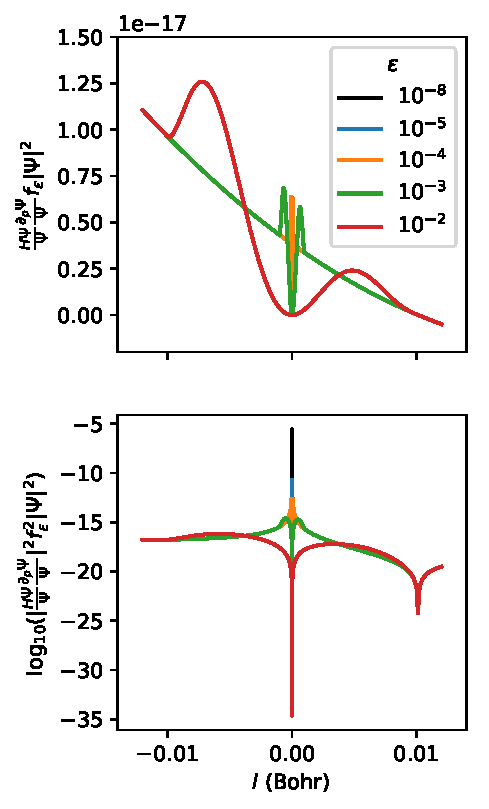
\includegraphics{../plots/viznode.pdf}
\caption{Logarithm of $Q * f_\epsilon$ and $(Q * f_\epsilon)^2$ plotted against the normal coordinate $r$ from a node of LiH. Curve colors correspond to different values of $\epsilon$ ranging from $10^{-1}$ to $10^{-8}$}
\end{figure*}

\begin{figure*}
\centering
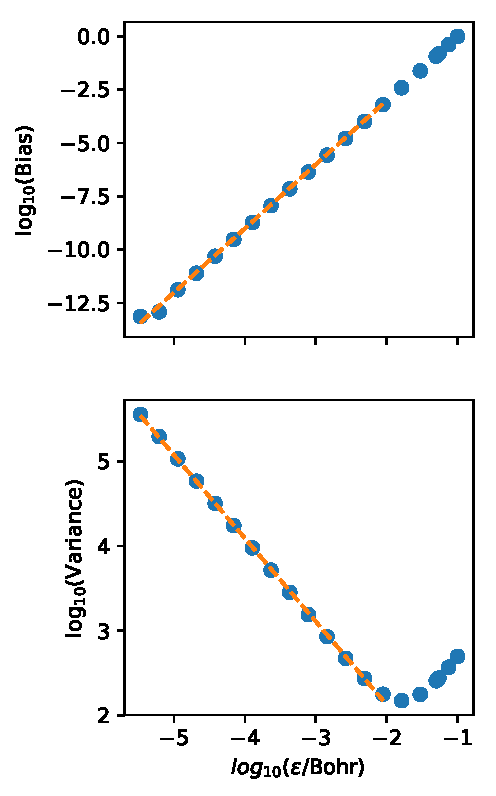
\includegraphics{../plots/integratenode.pdf}
\caption{Scaled bias and variance of Q evaluated by numerical integration from $r = -0.1$ to $r = 0.1$ across the node in Figure 1. The blue dots are the numerically integrated values and the orange curves indicate best fits to the functions $a\epsilon^3 + b$ and $c/\epsilon + d$ for the bias and variance, respectively.}
\end{figure*}

\end{document}